\documentclass[margin=14pt]{standalone}
\usepackage{tikz}
\usetikzlibrary{positioning}

\begin{document}
	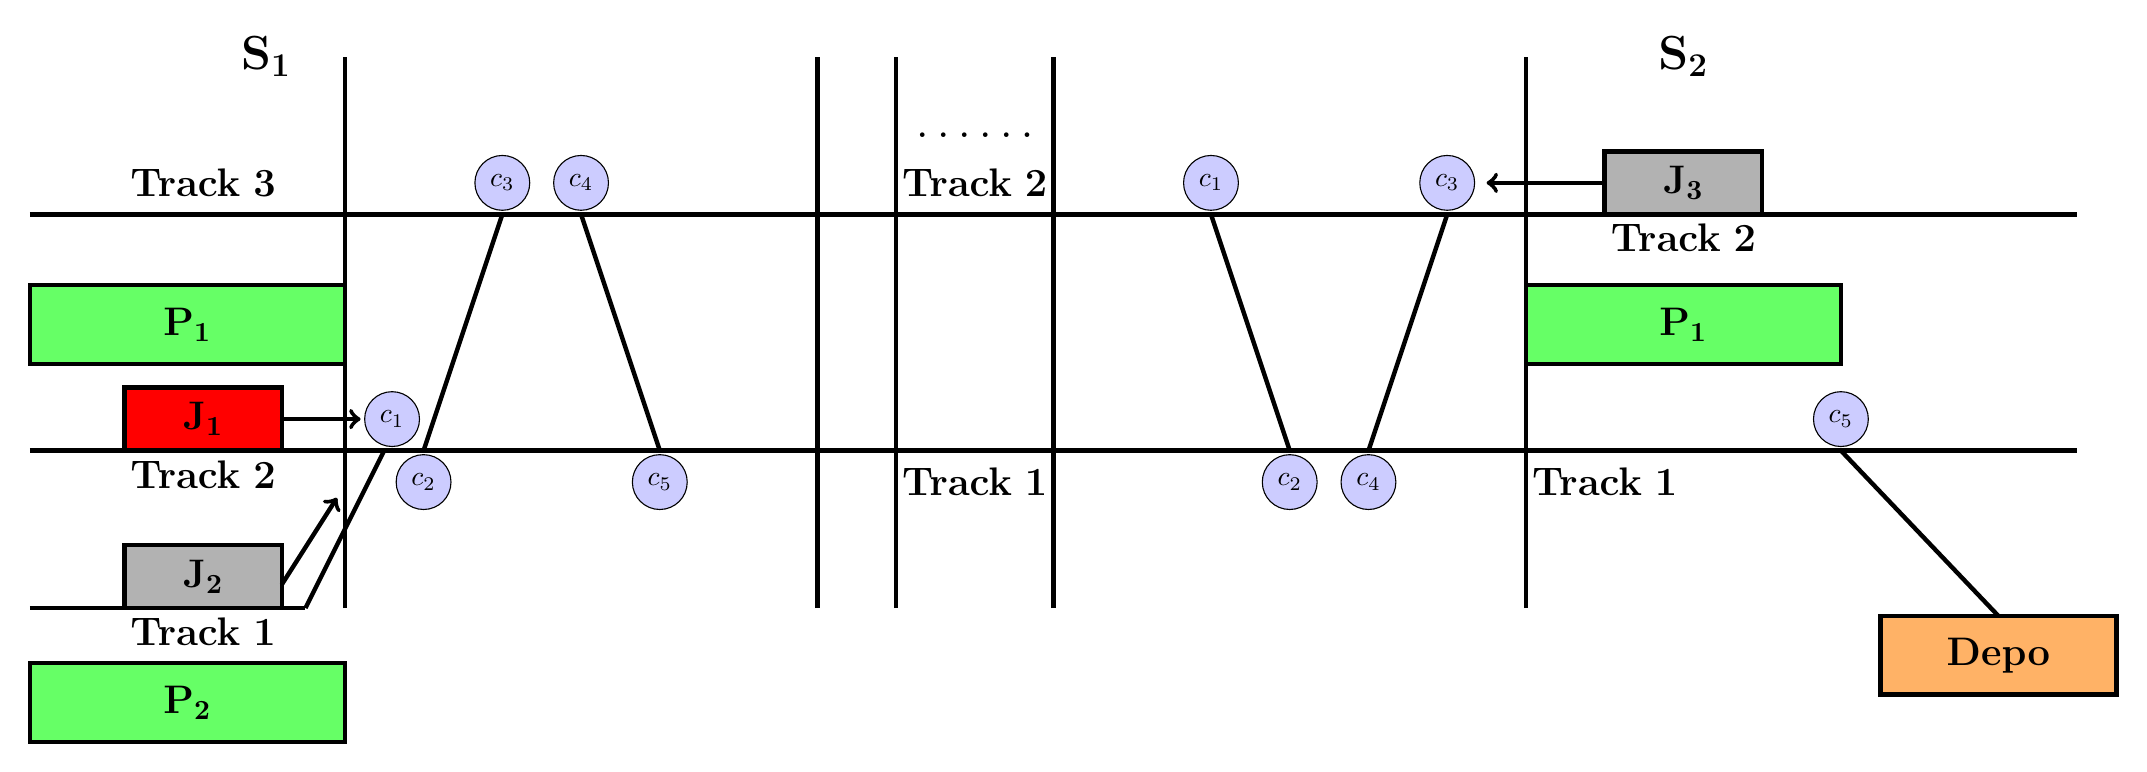
\begin{tikzpicture}[
	platform/.style={rectangle, draw=gray!80, fill=gray!20, very thick, minimum width=1.5cm, minimum height=0.8cm},
	fasttrain/.style={rectangle, draw=red!60, fill=red!20, very thick, minimum width=0.2cm},
	]
	%Nodes
	%\node[fasttrain]        (uppercircle)       [above=of maintopic] {1};
	%\node[squarednode]      (rightsquare)       [right=of maintopic] {3};
	%\node[roundnode]        (lowercircle)       [below=of maintopic] {4};
	\node[rectangle,
	draw = black,
	text = black, ultra thick,
	fill = gray!60, minimum width = 2cm, minimum height = 0.8cm] (r) at (-9.8,-1.6) {\Large$\mathbf{J_2}$};
	%
	\node[rectangle,
	draw = black,
	text = black, ultra thick,
	fill = gray!60, minimum width = 2cm, minimum height = 0.8cm] (r) at (9.,3.4) {\Large$\mathbf{J_3}$};
	%
	\node[rectangle,
	draw = black,
	text = black, ultra thick,
	fill = red!100, minimum width = 2cm, minimum height = 0.8cm] (r) at (-9.8,0.4) {\Large$\mathbf{J_1}$};
	%
	\node[rectangle,
	draw = black,
	text = black, ultra thick,
	fill = green!60, minimum width = 4cm, minimum height = 1cm] (r) at (-10,1.6) {\Large$\mathbf{P_1}$};
	%
	\node[rectangle,
	draw = black,
	text = black, ultra thick,
	fill = green!60, minimum width = 4cm, minimum height = 1cm] (r) at (-10,-3.2) {\Large$\mathbf{P_2}$};
	%
	\node[rectangle,
	draw = black,
	text = black, ultra thick,
	fill = green!60, minimum width = 4cm, minimum height = 1cm] (r) at (9,1.6) {\Large$\mathbf{P_1}$};
	%
	\node[rectangle,
	draw = black,
	text = black, ultra thick,
	fill = orange!60, minimum width = 3cm, minimum height = 1cm] (r) at (13,-2.6) {\Large$\textrm{\textbf{Depo}}$};
	%
	\node[circle,
	draw = black,
	text = black,
	fill = blue!20] (r) at (-7.4, 0.4) {$c_1$};
	%
	\node[circle,
	draw = black,
	text = black,
	fill = blue!20] (r) at (-7., -0.4) {$c_2$};
	%
	\node[circle,
	draw = black,
	text = black,
	fill = blue!20] (r) at (-4., -0.4) {$c_5$};
	%
	\node[circle,
	draw = black,
	text = black,
	fill = blue!20] (r) at (-6., 3.4) {$c_3$};
	%
	\node[circle,
	draw = black,
	text = black,
	fill = blue!20] (r) at (-5, 3.4) {$c_4$};
	%
	\node[circle,
	draw = black,
	text = black,
	fill = blue!20] (r) at (3, 3.4) {$c_1$};
	%
	\node[circle,
	draw = black,
	text = black,
	fill = blue!20] (r) at (6, 3.4) {$c_3$};
	%
	\node[circle,
	draw = black,
	text = black,
	fill = blue!20] (r) at (4, -0.4) {$c_2$};
	%
	\node[circle,
	draw = black,
	text = black,
	fill = blue!20] (r) at (5, -0.4) {$c_4$};
	%
	\node[circle,
	draw = black,
	text = black,
	fill = blue!20] (r) at (11, 0.4) {$c_5$};
	
	
	\draw [->, ultra thick](-8.8,0.4) -- (-7.8, 0.4);
	\draw [->, ultra thick](-8.8,-1.7) -- (-8.1, -0.6);
	\draw [->, ultra thick](8.,3.4) -- (6.5, 3.4);
	%
	\draw[ultra thick] (-7.5, 0) -- (-8.5, -2);
	\draw[ultra thick] (-12, -2) -- (-8.5, -2);
	%
	\draw[ultra thick] (-8, -2) -- (-8, 5);
	%
	\draw[ultra thick] (-12, 3) -- (14, 3);
	\draw[ultra thick] (-12, 0) -- (14, 0);
	%
	\draw[ultra thick] (-6,3) -- (-7,0);
	\draw[ultra thick] (-5,3) -- (-4,0);
	%
	\draw[ultra thick] (-2, -2) -- (-2, 5);
	\draw[ultra thick] (-1, -2) -- (-1, 5);
	\draw[ultra thick] (1, -2) -- (1, 5);
	%
	\draw[ultra thick] (3,3) -- (4,0);
	\draw[ultra thick] (6,3) -- (5,0);
	%
	\draw[ultra thick] (7, -2) -- (7, 5);
	%
	\draw[ultra thick] (11, 0) -- (13, -2.1);
	%
	\node[] at (-9.8, -2.3) {\Large\textbf{Track} $\mathbf{1}$};
	\node[] at (9, 2.7) {\Large\textbf{Track} $\mathbf{2}$};
	\node[] at (-9.8, -0.3) {\Large\textbf{Track} $\mathbf{2}$};
	\node[] at (-9.8, 3.4) {\Large\textbf{Track} $\mathbf{3}$};
	\node[] at (0, 3.4) {\Large\textbf{Track} $\mathbf{2}$};
	\node[] at (0, -0.4) {\Large\textbf{Track} $\mathbf{1}$};
	\node[] at (8, -0.4) {\Large\textbf{Track} $\mathbf{1}$};
	\node[] at (0, 4) {\LARGE$\ldots\ldots$};
	%
	\node[] at (-9, 5) {\LARGE$\mathbf{S_1}$};
	\node[] at (9, 5) {\LARGE$\mathbf{S_2}$};
	\end{tikzpicture}
\end{document}